\documentclass[conference]{IEEEtran}
\usepackage{cite}
\usepackage{amsmath,amssymb,amsfonts}
\usepackage{algorithmic}
\usepackage{graphicx}
\usepackage{textcomp}
\usepackage{xcolor}

\title{P21015: Fall Risk Mobile}

\author{\IEEEauthorblockN{Matt Krol}
\IEEEauthorblockA{mrk7339@rit.edu}
\and
\IEEEauthorblockN{Jacob DeFord}
\IEEEauthorblockA{jwd5062@rit.edu}
\and
\IEEEauthorblockN{Paul Kelly}
\IEEEauthorblockA{pjk2563@rit.edu}
\and
\IEEEauthorblockN{Doyle Bartholet}
\IEEEauthorblockA{cdb3120@rit.edu}}

\begin{document}

\maketitle

\begin{abstract}
Stroke is one of the leading causes of death and disability in the United States. Stroke survivors tend to have reduced motor functions, which puts them at higher risk of severe fall related injuries. At the time of writing, methods for assessing the fall risk of post stroke patients have been proposed, however, not many tools exist to collect the necessary data needed for these assessments in a practical and safe manner. In this paper, we propose a solution to the later that will allow post stroke patients to safely gather the data needed for fall risk evaluation from the location of their choice. Furthermore, our solution additionally allows post stroke patients to be assessed remotely once the necessary data has been gathered, eliminating the need for travel.
\end{abstract}

\section{Introduction and Problem Statement}

In the United States, someone has a stroke every 40 seconds and someone dies from a stroke every 4 minutes \cite{virani2020heart}. Among the many challenges that post stroke patients face, fall related injuries are among the most common and can occur at any point of a post stroke patients daily routine. Studies have shown that chronic stroke patients fall at rates between 23\% and 50\%, with many patients reporting significant injury after such falls \cite{harris2005relationship}. For this reason, many post stroke patients are assisted by caretakers or family members which can cause emotional stress and financial problems, among others. Therefore, it is critical that a post stroke patient and their family have all of the tools necessary to make an informed decision about how the post stroke patient is to be cared for. At the time of writing, many researchers are attempting to develop a quantitative fall risk scale. This fall risk scale would be an important tool for post stroke patients and their families to determine the appropriate precautions and care needed.

There are many challenges associated with developing such a fall risk scale. One of these challenges being that data must be collected from post stroke patients in order for them to be evaluated. While survey data is easy to obtain via a variety of different methods, the motion sensor data needed for many fall risk models would require specialized equipment and supervision, which is likely only available at a medical facility. For many post stroke patients, leaving their home or care facility can put them at an even higher risk of falling--not to mention--collecting data in a different location can result in inaccurate or unrealistic data used as input to the fall risk model which reduces the quality of the result. Another challenge is the delivery of the fall risk results. In many cases, a fall risk evaluation can help prevent injury or even death. This is why it is important that the fall risk result is communicated in an efficient and streamlined manner to all necessary parties as soon as the results become available.

In this work, we will focus on solving the problem of collecting and transmitting the data necessary for a fall risk evaluation and the problem of communicating the fall risk results back to the post stroke patient and other necessary parties. Our work is independent of the actual fall risk model. We hope that our framework will be widely adopted by different researchers developing different models for fall risk evaluation. 

We will first discuss the proposed solution and design, then the feasibility of the design and benchmarks. We will follow up with concluding remarks and future development opportunities. 

\section{Proposed Solution and Design}

In this section, we will discuss the overall architecture. Then, we will discuss each of the three components in detail. The three components are the mobile application, the web server, and the Matlab API. 

\subsection{High Level Solution}

\begin{figure}[!htb]
\centering
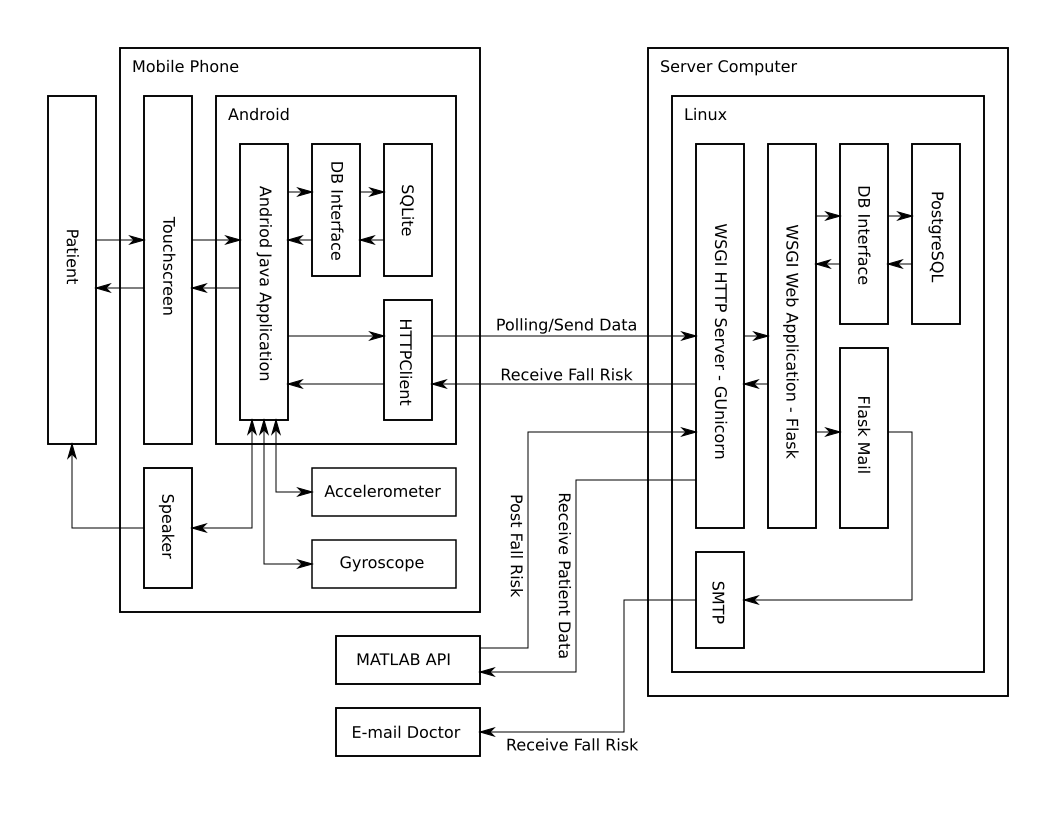
\includegraphics[scale=0.3]{img/systemdesign.png}
\caption{System Level Design}
\label{systemleveldesign}
\end{figure}

Collecting and transmitting fall risk data requires several technologies. First, the data must be collected using motion sensors attached to the patient. The motion sensors should be easily controllable by the patient so that no training is required to take the assessment. Next, the data must be transmitted digitally to a storage device that can be accessed by the researchers. The storage device should be easily accessible from Matlab, since the fall risk metrics will be calculated using Matlab. The storage device should also be able to hold data from many different patients in an organized manner.

Figure \ref{systemleveldesign} shows the proposed overall system level design. The solution is broken down into three main components: a mobile application, a web server, and a Matlab API. The smart phone application was chosen for it's rapid development, ease-of-use, and built-in motion sensors. Modern smart phones provide both the motion sensors required and the easy-to-use interface required by the patient-side device. Most patients will likely have a smart phone, and a free mobile application is accessible by anyone with an Android phone. The web server was designed to provide a universal API that is easily accessible from any device while still providing some security. The API provides an interface to a database that stores all of the patient data in an organized manner. The API's simple design allows for the Matlab API to also be very simple. All the Matlab script needs to do is format HTTP requests. This design effectively collects patient data in an easily-controlled manner, sends it to an easily-accessible storage device, and provides the information to virtually any internet-connected computer, including the researcher's Matlab device.

\subsection{Android Mobile Application}
The mobile application development was broken up into two parts: the front end and the back end. This section will first discuss the front end GUI, then the back end data management and networking.

The front end of the application involves the layout of activities and the content of these activities. Activities are essentially the pages of the app, a button can navigate the user to a different screen. Each of those screens is an activity with its own texts and buttons. Some parts of this layout were given by the customer such as the number of tests and survey questions. The rest of the layout was created using initiative and customer feedback.

The back end of the application follows a simple process. All networking is done through HTTP requests, starting with the user login. When the user logs in with an existing account, the application stores a single authentication token to be sent back to the server for all future requests. If the user does not have an account, the application submits account creation data to the server to allow the user to login and obtain an authorization token. 

After logging in, the user can navigate to either the information survey or the data collection tests. The survey information is collected as strings and submitted to the server as a large JSON string in an HTTP request. The request must include the user's authentication token or the request will be ignored. Likewise, the information from the physical tests must be submitted with the token or else it will be ignored.

The data collection tests involve both manipulating the phone's motion sensors and submitted the collected data to the server. Standard Android phones come with a gyroscope and an accelerometer. The Android operating system provides several higher-level sensor classes that automatically format the data into nice formats, such as a step counter or rotational velocity sensor. There are seven specific motion data objects: an accelerometer, gyroscope, gravity sensor, linear accelerometer, rotational velocity sensor, and step counter. Every time a sensor is read, it creates a simple object of the sensor's data points at that instance in time. So, during a test, the sensors are read continuously to populate an array for that test. Each sensor array is collected into a single data manager object which is serialized and stored locally on the phone. Once the test is complete, the serialized object is encoded in base64 and sent to the server in a JSON string where it is stored in the data base for the given user. 


\subsection{Flask Web Server}

The HTTP REST API implemented on our web server is a key subsystem in our overall system design. This is because the HTTP REST API is what will handle bidirectional communication between the research team and the clients on their mobile application. The term HTTP refers to the application level internet communication protocol. The HTTP internet communication protocol has been a mainstay of the internet since the beginning of its existence and is still widely in use today. The term REST refers to a standardized interface for creating web services. We will follow the convention of using the JSON text format for sending and receiving information via the REST API. The main feature of a REST API is that it is stateless, which greatly simplifies the implementation. Finally, in our web server we must also utilize a relational database to store user profile information, survey data, tests data, and also fall risk results.

The main function of our REST API is to create a bidirectional communication loop between the clients on the mobile application and the research team. The database will store the necessary profile, tests, and survey information. A typical usage scenario of the REST API is as follows:
\begin{enumerate}
\item Client creates a profile via the REST API
\item Client requests a temporary login token via the REST API.
\item Client collects survey and test data via the mobile application.
\item Client sends the survey and test data to the be stored in the web server database via the REST API.
\item Researchers pull survey and test data from the web server database via the REST API.
\item Researchers analyze data and evaluate fall risk.
\item Researchers post fall risk results to the database via the REST API.
\item Client pulls fall risk evaluation data from the database via the REST API.
\item Repeat if necessary by going back to step 2.
\end{enumerate}
In addition to implementing the REST API calls needed for the steps above, we also will implement REST API calls for the clients to:
\begin{itemize}
\item Edit their profile information, i.e., change their e-mail address, password, etc.
\item Delete their profile, survey, and test information.
\item Reset their password in case they forget it.
\item Revoke a temporary access token.
\end{itemize}

For our database in the web server we can use one of the standard SQL relational database implementations. We will use a single table with the following columns:
\begin{itemize}
\item \texttt{id}: The unique integer id of a user.
\item \texttt{firstname}: The string first name of a user.
\item \texttt{lastname}: The string last name of a user.
\item \texttt{email}: The unique string email address of a user.
\item \texttt{admin}: A boolean flag indicating if a user has admin privileges or not.
\item \texttt{creation\_timestamp}: A datetime object containing the creation date of the user account.
\item \texttt{modification\_timestamp}: A datetime object containing the date that the user account was last modified. Defaults to the creation\_timestamp value.
\item \texttt{survey}: A JSON string containing a the survey data of a user.
\item \texttt{survey\_timestamp}: A datetime object containing the date of the last survey that the user took. This value can be None.
\item \texttt{tests}: A binary blob containing the serialized Java class that should contain the tests data of a user. This value can be None.
\item \texttt{tests\_timestamp}: A datetime object containing the date of the last tests that the user took. This value can be None.
\item \texttt{result}: A JSON string containing the fall risk result. This value can be None.
\item \texttt{result\_timestamp}: A datetime object containing the date of the last result that was posted.
\item \texttt{password\_hash}: A string containing the user hashed password.
\item \texttt{token}: A string that contains a user temporary access token.
\item \texttt{token\_expiration}: A datetime object that contains the expiration date of a user token.
\end{itemize}
Each user will be stored in a row of the database. The above fields will allow us to store the necessary user profile information, survey data, tests data, and fall risk results. Several timestamps allow us to determine whether or not a user has posted recent tests and survey information so they can be evaluated.

Lastly, our web service must have some sort of authentication system. The REST API endpoints that are used by each respective user via the mobile application should be private, i.e., users should only be able to modify or see resources in the database that belong to them. Secondly, all REST API endpoints used by the researchers should be sufficiently locked down and they should not be publicly accessible. Effectively, the researcher accounts will be administrator accounts. In the database, administrator accounts will be identified by the admin flag. This flag can only be set manually by a server maintainer for security purposes. Each of the REST API endpoint categories described will utilize a temporary access token that will expire after one hour. So users must first create an account, and then request a temporary access token in order to further obtain or modify resources in the database.

\subsection{MATLAB Java API}
The Matlab Java API should provide an easy-to-use program that allows the researchers to interact with the web server containing the user database. Some possible designs include using a Matlab HTTP library to send and receive data, or an integrated Java application that can be called from Matlab. The design should make it easy to package data for transmission over the internet as well as use a package format that can be used by both Matlab and Android. 

Since both Matlab and Android are closely integrated with standard Java, Java class serialization can be leveraged to transmit and store the user data. On the Android side, the physical sensor data is packaged into a data manager class that holds all of the information for a given test. This class can be serialized and stored as serialized data in the database. Then, the Matlab script must de-serialize the class in order to access the data. 

We propose a Java application that provides an API that makes interacting with the web server simple from Matlab. The Java application, installed with precompiled classes, can be called from a Matlab script and can provide the necessary user data with little effort. A sample Matlab script will be included to demonstrate the functionality of the Java application.

\section{Design Feasibility and Benchmarks}

This section will discuss the specifics of the implementation and benchmarks.

\subsection{Android Mobile Application}
This section will discuss some of the difficulties of implementing the Android application. 

The first part for creating the front end of the application is to create the layout. For the first iteration of the front end application layout Thunkable was used. This website has a lot of tools to rapidly prototype android applications and was used to create the initial demo layout and flow for the application. This application was demoed with the customer and was received very positively. With the initial application layout and activity flow created, the entire workflow was recreated using Android Studio. Android Studio is an IDE developed by Google to program applications for Android. This IDE had a very useful activity designer for designing the XML for each activity. Figure \ref{thunkvsandroid}, below, shows the variation between these activities in each development environment.

\begin{figure}[!htb]
\centering
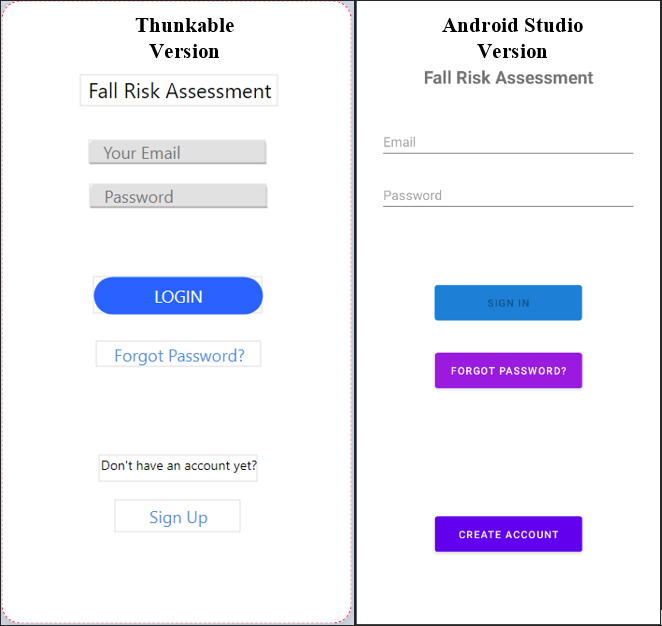
\includegraphics[scale=0.5]{img/Thunkable_vs_android_studio.png}
\caption{Thunkable versus Android Studio Activity}
\label{thunkvsandroid}
\end{figure}

One problem with developing for Android is that you have to make the app usable for all types of phones, Android Studio does this by constraining elements of the GUI to other parts of the activity. This makes it so parts can scale of each other to accommodate for different sized screens. This scaling feature was not realized when the entire application was programmed in Android Studio. Because of this, the entire framework of the GUI layout for each activities had to be reprogrammed. While this caused some problems, it has allowed the application to be usable on all screen sizes.

The back end of the application also faced some difficulties. The sensor data collection implementation was simple. However, when trying to submit information to the server, several issues arose. First, Android restricts networking on the main application thread because any networking delay can freeze the entire application. In development, this warning was disabled to prove functionality and then re-enabled for the final solution. 

Another issue we faced in developing the networking for the application was managing a secure token. Each page (or activity) in an Android app is a separate instance of a Java object so information must be passed from page to page. In order to provide the authentication token across several activities, the token must be explicitly passed to every activity that is launched. This provided an effective solution for storing the token in the application across activities. 

\subsection{Flask Web Server}

There are several so called web stacks for implementing web services. Given that our team has more experience using Python, we decided to use a Python based web stack. A Python web stack consists of a HTTP server, application server, Python web framework, and a relational database. We decided to use the very popular Flask web framework, along with PostgreSQL for our database and gunicorn for our combined HTTP and application server. All of these tools are open source and have been vetted by the open source community and industry, not to mention, they have been in use for around a decade. Additionally, all of these tools are widely documented and follow all of the standard protocols such as HTTP, PEP, TCP/IP, REST, etc. This not only allows us to focus on our higher level design, but it 
lows our design to scale if needed to include other standardized services. Finally, we also needed a computer to run our services on. We were able to obtain a virtual machine from RIT to run our web service on. This virtual machine is running the Linux operating system which is ideal for deploying our web service. We utilized Docker to automate the deployment process.

In particular, our implementation was highly influenced by \cite{grinberg2018new}. The author in \cite{grinberg2018new} also developed many Flask extensions that we used to implement e-mail services (Flask-Mail), token and basic HTTP authentication (Flask-HTTPAuth), among others. The author in \cite{grinberg2018new} is widely known in the Python web service community, and his Flask extensions have been vetted by the open source community. Hence, because we are utilizing standardized and community vetted tools, we feel that our implementation is feasible. Mobile applications and web services are so common these days that many resources and tools exist to aid developers and we have tried to take advantage of this. At the time of writing we have been able to implement the main design requirements of our HTTP REST API, namely, the communication loop. While most of the testing has been manual, we believe that this is strong evidence that our design is feasible and will meet the demands of our client.

\subsection{MATLAB Java API}

The Matlab Java API was split up into two main components: the Java application and the Matlab script. The Java application includes a main FallRiskAdmin class that provides functions that can interact with the server. These functions include a getToken() function, that logs in and sets the authentication token for future requests. It also has a getUserData function that pulls all of the stored data about a single user. Finally, there is a postUserResults function that sends the results of the data analysis back to the server for review by the user. There are several object classes as well, including a TokenResp class that holds the token information and UserData and UserResult classes that hold data for the user in the local Java application.

This Java application is designed to be callable from a Matlab script. The installation of the Java application includes a sample example.m Matlab script that demonstrates how to call the Java program from Matlab. This is a very simple script that uses the Java program to log in to the web server to obtain a token, then pull and send sample user data. It should be everything the researchers need to interact with the server we have set up. 

\section{Next Steps}

\subsection{Flask Web Server}

While the web server in its current state is fully functional, there are some improvements that should be implemented:

\begin{itemize}
    \item Upgrade the web server to use HTTPS instead of HTTP. The use of HTTPS is standard these days as it encrypts message information while in transit. Regular HTTP transmits message information in plain text.
    \item Use a professional e-mail server on the server computer. At the time of writing, we are using a gmail account to send e-mails. In order to deploy a professional e-mail server on the server computer and to have the messages be able to be received by major e-mail providers, an e-mail relay must be set up. In order to setup a Google e-mail relay, a professional google account is needed (an RIT gmail account would suffice).
    \item Once the professional e-mail server is in place, there should be an e-mail validation step before a user is allowed to create an account. This will prevent users from being locked out of their accounts, and it will also prevent someone from maliciously overloading the database with invalid accounts.
    \item Setup a proxy server, e.g., something like NGNIX to sit in front of gunicorn. In addition to load balancing and caching, the proxy server will act similar to a firewall in that it will prevent direct access to the internal resources of the server (this can prevent DOS attacks).
\end{itemize}

\subsection{Mobile Application}

\subsection{MATLAB Java API}

\section{Conclusion}

The overall goal of this project has been to create a tool that can collect the necessary data needed for fall risk evaluation from post stroke patients and to also allow for post strokes patients to have their fall risk evaluated remotely by a research team. Our solution was to create an Android mobile application, web service, and MATLAB API. The mobile application will provide the interface for post stroke patients to collect important biometric and categorical data that is needed for a fall risk evaluation. In addition, the mobile application is how post stroke patients will communicate with the research team. At the heart of this bidirectional communication loop between the researchers and the post stroke patients on their mobile application is our web service. Our web service was implemented via industry standard software libraries and database implementations. Lastly, since our research team uses MATLAB for their fall risk model, we have implemented a MATLAB API to interact with our web service, thus, completing the communication loop between the post stroke patient and research team. This bidirectional communication loop between the post stroke patients and research team allows post stroke patients to be safely evaluated for fall risk from the comfort of their own home, and with or without the help of a family member or caretaker. Thus, our product can prevent potentially fatal fall related injuries. Furthermore, our solution is flexible and is implemented with standardized tools, so it can be easily extended or be utilized by other research teams. We hope that our product will have a positive impact on the community of post stroke patients and the teams that work hard to create accurate fall risk models.

\bibliographystyle{IEEEtran}
\bibliography{bibliography}

\end{document}
